% -*-latex-*-
%\documentclass[handout]{beamer}
\documentclass[12pt]{beamer}
\usepackage{etex}

\let\latexput\put
\usepackage{pictex}
\let\pictexput\put
\let\put\latexput

\usepackage{color}
%\setbeamercovered{transparent}
%\usepackage{pst-plot,color,pstricks}
%\setlength{\topmargin}{-1.7in}
\setbeamertemplate{footline}[frame number]
\begin{document}
\title{Selection at Two Loci}
\author{Alan R. Rogers}
\date{\today}
\frame{\titlepage}

\frame{\frametitle{Model with random mating, no selection}

{\centering\fbox{\begin{minipage}{0.7\textwidth}
\begin{eqnarray*}
x_1 &=& \hbox{frequency of $AB$-gametes}\\
p_A &=& \hbox{frequency of $A$-gametes}\\
p_B &=& \hbox{frequency of $B$-gametes}\\
c   &=& \hbox{probability of recombination}
\end{eqnarray*}
\end{minipage}}\\}

\bigskip

Change in frequency of $AB$-gametes during one generation:
\[
x'_1 = x_1 -cD
\]
}

\frame{\frametitle{All four gametes, still no selection}
\[
\begin{array}{crcl}
\hbox{Gamete}     & \multicolumn{3}{c}{Recurrence}\\
AB & x'_1 &=& x_1 -cD\\
Ab & x'_2 &=& x_2 +cD\\
aB & x'_3 &=& x_3 +cD\\
ab & x'_4 &=& x_4 -cD\\
\end{array}
\]
}

\frame{\frametitle{Selection affecting gametes}
\[
\begin{array}{crcl}
\hbox{Gamete}     & \multicolumn{3}{c}{Recurrence}\\
AB & x'_1 &=& w_1 (x_1 -cD)/\bar w\\
Ab & x'_2 &=& w_2 (x_2 +cD)/\bar w\\
aB & x'_3 &=& w_3 (x_3 +cD)/\bar w\\
ab & x'_4 &=& w_4 (x_4 -cD)/\bar w\\
\end{array}
\]
where $\bar w = \sum x_i w_i$ is mean fitness.

\bigskip

\pause
What if selection acts on adults?
}

\begin{frame}
\frametitle{The effect of recombination}

What gametes are produced by the following genotypes?
\[
\begin{array}{lccccc}
 & \hbox{Heterozygous}      & \multicolumn{4}{c}{\hbox{Gametes produced}}\\
\hbox{Genotype}& \hbox{loci} & AB & Ab & aB & ab\\
AB/AB & 0 & \pause 1 \\
\pause AB/Ab& 1
         & \pause 1/2&1/2\\
\pause AB/ab & 2
         & \pause \frac{1-c}{2}&\frac{c}{2} &\frac{c}{2}&\frac{1-c}{2}\\
\pause Ab/aB & 2
         & \pause \frac{c}{2}&\frac{1-c}{2} &\frac{1-c}{2}&\frac{c}{2}\\
\end{array}
\]
\pause
Only double heterozygotes make recombinant gametes.

\medskip

If these genotypes have low fitness, few recombinants appear.
\end{frame}

\frame{\frametitle{Selection affecting diploid adults}
\[
\begin{array}{crcl}
\hbox{Gamete}     & \multicolumn{3}{c}{Recurrence}\\
AB & x'_1 &=& \bar w_1 (x_1 -c w_h D)/\bar w\\
Ab & x'_2 &=& \bar w_2 (x_2 +c w_h D)/\bar w\\
aB & x'_3 &=& \bar w_3 (x_3 +c w_h D)/\bar w\\
ab & x'_4 &=& \bar w_4 (x_4 -c w_h D)/\bar w\\
\end{array}
\]
\begin{itemize}
\item<2->Fitnesses become $\bar w_i$: weighted mean over genotypes in which
  gamete $i$ appears.
\item<3->Recombination limited by the fitness $(w_h)$ of double
  heterozygotes: only these contribute recombinant
  gametes.
\item<4->Useful as a recipe for calculation.
\end{itemize}
}

\begin{frame}
\frametitle{$A$ sweeps; $B$ hitch-hikes}
\framesubtitle{Parameters: $s=0.02$, $c=0.001$, $N=5000$}
\begin{columns}
\column{0.6\textwidth}
\includegraphics[width=\textwidth]{twolocsim2.pdf}
\column{0.35\textwidth}<1->
\color{red}
Selective sweep of allele $A$.

\medskip\color{green}
Allele $B$ hitch-hikes to fixation.

\medskip\color{blue}
$D$ high when $p_A$ has high heterozygosity.

\medskip\color{violet}
$d$ high throughout
\end{columns}
\end{frame}

\begin{frame}
\frametitle{Linked allele may fail to increase}
\framesubtitle{Parameters: $s=0.02$, $c=0.001$, $N=5000$}
\begin{columns}
\column{0.65\textwidth}
\includegraphics[width=\textwidth]{twolocsim.pdf}
\column{0.35\textwidth}<1->
\onslide<1->\color{red}
Allele $A$ sweeps to fixation.

\medskip\color{green}
Little change in linked allele.  Why?

\medskip\color{blue}
LD lost early on this run, so $D$ near 0.

\medskip\color{violet}
Loss of LD shows as big drop in $d$.
\end{columns}
\end{frame}

\begin{frame}
\begin{columns}
\column{0.6\textwidth}
 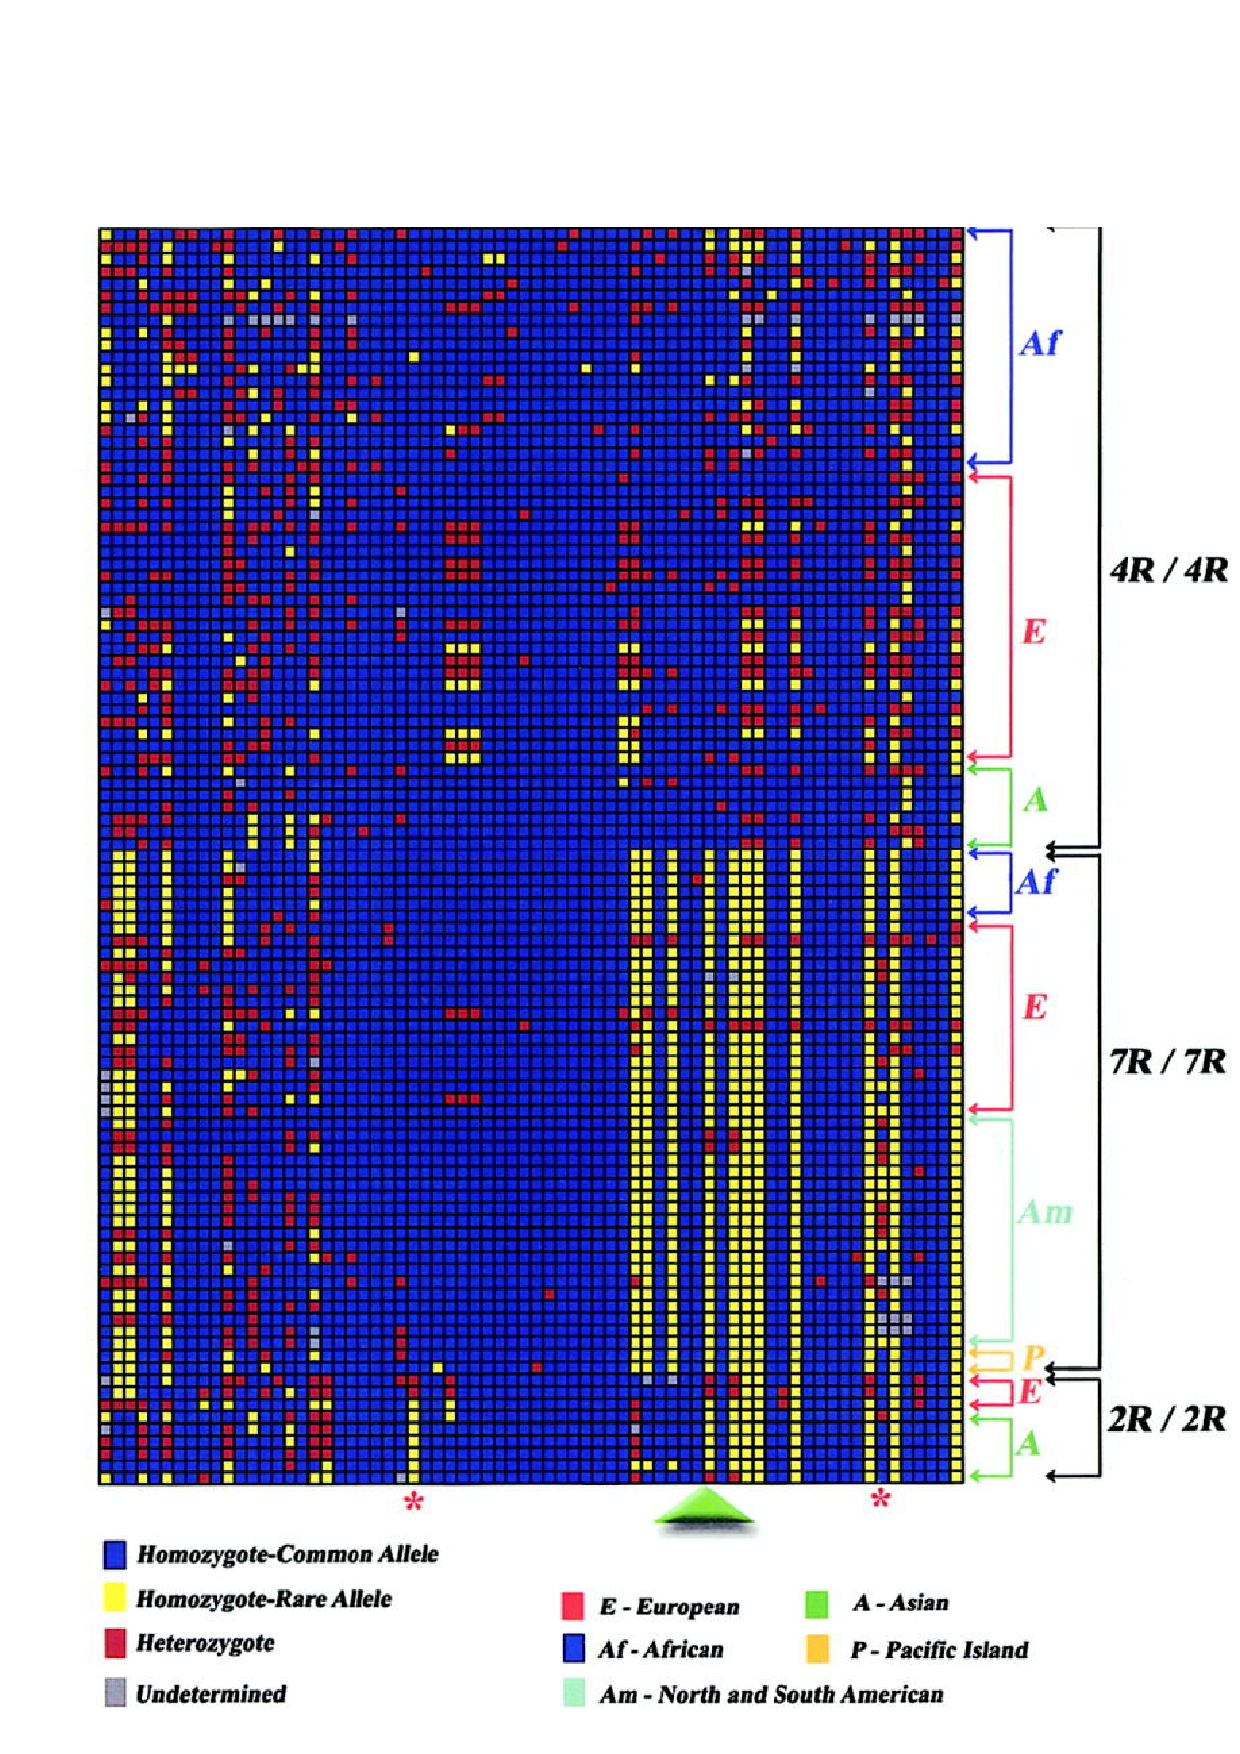
\includegraphics[height=0.9\textheight]{drd4-polymorph.pdf}
\column{0.4\textwidth}\raggedright
\begin{itemize}
\item LD at D4 dopamine receptor
\item Rows are diploid genotypes
\item Blue: common homozygote
\item Yellow: rare homozygote
\item Red: heterozygote
\item Note LD w/i 7R genotypes
\end{itemize}
\end{columns}
\end{frame}

\begin{frame}
\frametitle{DNA sequences from region of human lactase gene}
%DNA sequences near human lactase gene, typed in a
%European sample.  Columns are
%nucleotide sites.  Top row (the
%reference sequence) shows common state at each site. Capital
%\texttt{A} is lactase persistance
%allele\cite{Bersaglieri:AJH-74-1111}.  Numbered rows represent
%individual chromosomes. Dots indicate identity with top row.  60
%chromosomes identical to reference sequence were omitted to save
%space. From HapMap release r23.}\label{tab.lctseq}
%
\tiny
\centering
\ttfamily
\begin{tabular}{cc}
  &cgcttcaggcattcctatctaaacagaccaacgtaAgggtacaatgcctaacccagacgtttcaactct\\
20&.....................................................................\\
21&.....................................................................\\
22&.....................................................................\\
23&.....................................................................\\
24&.....................................................................\\
25&.....................................................................\\
26&.....................................................................\\
27&..................t..................................................\\
28&..................t..................................................\\
29&..................................................c..................\\
37&...................................G..a.gt.....t.........gac.c.tgtct.\\
38&...ccgga....gat..at..gg..c.....tc.gGaaa.g..ccttt...tg......c...t.t...\\
39&...ccgga....gat..at..gg..c.....tc.gGaaa.g..ccttt...tg......c...t.t...\\
40&..tcc...agtag.t.cat..g.....t..ttccgG..a.gt.....t.........gac.c.tgtct.\\
41&..tcc...agtag.t.cat..g.....t.gttccgG..a.gt.....t.........gac.c.tgtct.\\
42&..tcc...agtag.t.cat..g.....t.gttccgG..a.gt.....t.........gac.c.tgtct.\\
43&..tcc...agtag.t.cat..g.....t.g.tc.gG..a.gt.....t.........gac.c.tgtct.\\
44&..tcc...agtag.t.cat..g.....t..ttc.gG..acgt.....t.........gac.c.tgtct.\\
45&..tcc...agtag.t.cat..g.....t.gttc.gG..a.gt.....t.........gac.c.tgtct.\\
46&...ccgga....gat..at..gg..c.....tc.gGaaa.g..ccttt...tg......cg.gt.t..c\\
47&..tcc...agtag.t.cat..g.....t.gttccgG..a.gt.....t.........gac.c.tgtct.\\
48&..tcc...agtag.t.cat..g.....t.gttccgG..a.gt.....t.........gac.c.tgtct.\\
49&..tcc...agtag.t.cat..g.....t.gttccgG..a.gt.....t.........gac.c.tgtct.\\
50&tatccgga....g.tc.atcgg.tc.g.tg.tc.gG..a.g.g....tg....ggt...cg.gt.t..c\\
51&ta.ccgga....g.t..atcgg.tc.g.tg.tc.gG..a.g.g....tg....ggt...cg.gt.t..c\\
52&ta.ccgga....g.t..atc.g.tc.g.tg.tc.gG..a.g.g....tg....ggt...cg.gt.t..c\\
53&ta.ccgga....g.t..atcgg.tc.g.tg.tc.gG..a.g.g....tg....ggt...cg.gt.t..c\\
\end{tabular}
\end{frame}

\begin{frame}
  \frametitle{Summary}
  \begin{itemize}
    \item Two-locus gametic selection is very simple.
    \item When selection acts on diploids, the recombination rate is
      weighted by the fitness of double heterozygotes.
    \item Hitch-hiking: selection at one locus may change allele
      frequencies at linked loci.
    \item If enough recombination happens early in the process, linked
      loci do not hitch-hike.
  \end{itemize}
\end{frame}  

\end{document}
